\newpage
\section {Билет 10. Методы обеспечения отказоустойчивости. RAID, распределенное хранение данных, виды и репликаций.}
\subsection {RAID}
RAID (Redundant Array of Independent Disks) - технология повышения отказоустойчивости и производительности дисковой подсистемы. Основная идея технологии заключается в распределении информации по массиву дисков с вычислением контрольных сумм. Поэтому в случае выхода из строя одного диска данные могут быть восстановлены с помощью информации, находящейся на других дисках. 
Выделяют несколько уровней (типов) RAID.

\begin {itemize}
\item RAID 0. \\
Информация разбивается на блоки данных $A_{i}$ фиксированной длины и записывается на несколько дисков поочередно. На картинке приведен пример с двумя дисками, но логически они составляют один диск. 
Достоинства:
\begin {itemize}
\item Скорость считывания файлов увеличивается в n раз, где n — количество дисков. При этом такая оптимальная производительность достигается только для больших запросов, когда фрагменты файла находятся на каждом из дисков.
\end {itemize}

Недостатки:
\begin {itemize}
\item При выходе из строя одного диска, информацию, которая на нем хранилась никак не восстановить.
\end {itemize}


\begin{figure}[h!]
\begin{minipage}[h]{0.3\linewidth}
\center{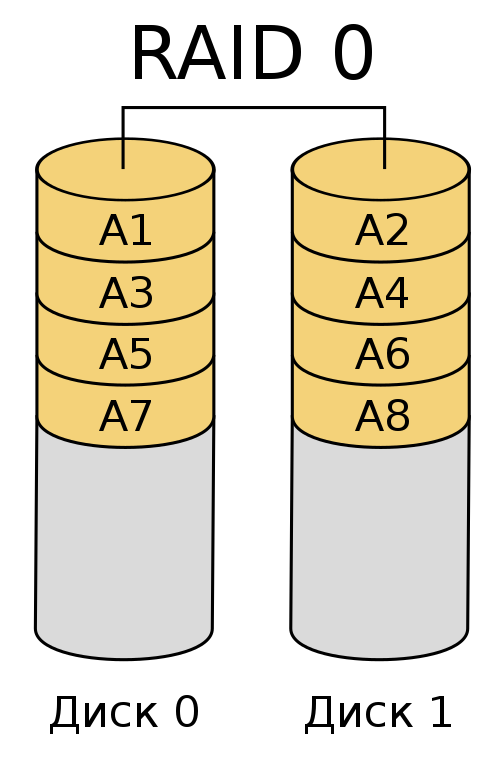
\includegraphics[width=0.5\linewidth]{10/0}}
\end{minipage}
\hfill
\begin{minipage}[h]{0.3\linewidth}
\center{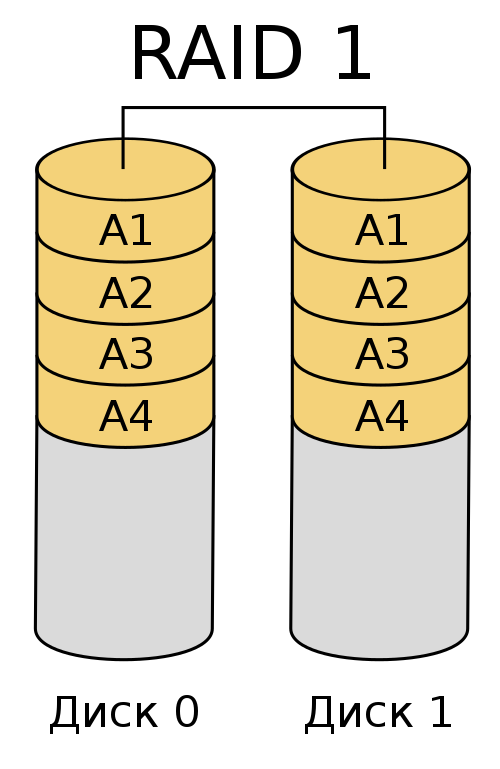
\includegraphics[width=0.5\linewidth]{10/1}}
\end{minipage}
\hfill
\begin{minipage}[h]{0.3\linewidth}
\center{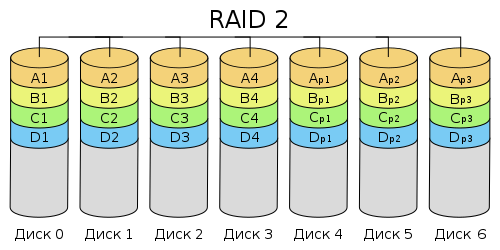
\includegraphics[width=\linewidth]{10/2}}
\end{minipage}
\end{figure}

\item RAID 1. \\
Массив из двух (или более) дисков, являющихся полными копиями друг друга. (Все диски объединяются в пары и дублируют информацию).
Достоинства:
\begin {itemize}
\item Обеспечивает приемлемую скорость записи (такую же, как и без дублирования) и выигрыш по скорости чтения при распараллеливании запросов.
\item Имеет высокую надёжность — работает до тех пор, пока функционирует хотя бы один диск в массиве.
\end {itemize}

Недостатки:
\begin {itemize}
\item При формальном количестве $2n$ дисков пользователь фактически получает только $n$.
\end {itemize}

\item RAID 2. \\
На лекции про него не говорили, но для порядка опишем этот подход. Массивы такого типа основаны на использовании кода Хэмминга. Диски делятся на две группы: для данных и для кодов коррекции ошибок, причём если данные хранятся на $2^n - n- 1$ дисках, то для хранения кодов коррекции необходимо $n$ дисков. Суммарное количество дисков при этом будет равняться $2^n - 1$. Данные распределяются по дискам, предназначенным для хранения информации, так же, как и в RAID 0, то есть они разбиваются на небольшие блоки по числу дисков. Оставшиеся диски хранят коды коррекции ошибок, по которым в случае выхода какого-либо жёсткого диска из строя возможно восстановление информации. Недостатком массива RAID 2 является то, что минимальное количество дисков, при котором имеет смысл его использовать — 7.

\item RAID 3. \\
Вспомним для начала, что такое XOR (исключающее ИЛИ, оно же сложение по модулю 2). Главное свойство этой операции в том, что если 
$a \oplus b = c$, то $c \oplus b = a$ так как $(a \oplus b) \oplus b = a \oplus (b \oplus b) = a$ (c b аналогично). \\
Применим эту идею. Разделим информацию на куски размером меньше сектора (разбиваются на байты), если следовать картинке то получим: $A_1, A_2 ... A_6, B_1, B_2 ... B_6$. На первые три диска последовательно запишем блоки информации, а на последний $A_1 \oplus A_2 \oplus A_3$, $A_4 \oplus A_5 \oplus A_6$ и т.д. Тем самым, если выйдет из строя диск 2, то с помощью рассмотренного выше свойства получим утерянную информацию.
Достоинства:
\begin {itemize}
\item высокая скорость чтения и записи данных;
\item минимальное количество дисков для создания массива равно трём.
\end {itemize}

Недостатки:
\begin {itemize}
\item массив этого типа хорош только для однозадачной работы с большими файлами, так как время доступа к отдельному сектору, разбитому по дискам, равно максимальному из интервалов доступа к секторам каждого из дисков. Для блоков малого размера время доступа намного больше времени чтения;
\item большая нагрузка на контрольный диск, и, как следствие, его надёжность сильно падает по сравнению с дисками, хранящими данные.
\end {itemize}

\begin{figure}[h!]
\begin{minipage}[h]{0.3\linewidth}
\center{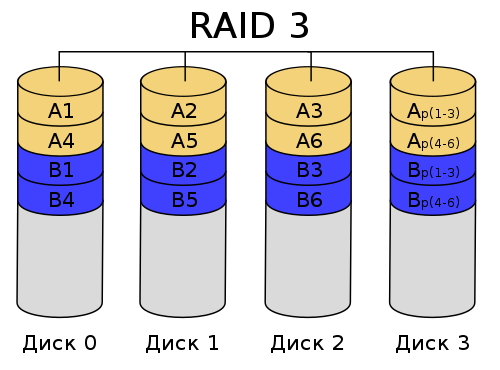
\includegraphics[width=\linewidth]{10/3}}
\end{minipage}
\hfill
\begin{minipage}[h]{0.3\linewidth}
\center{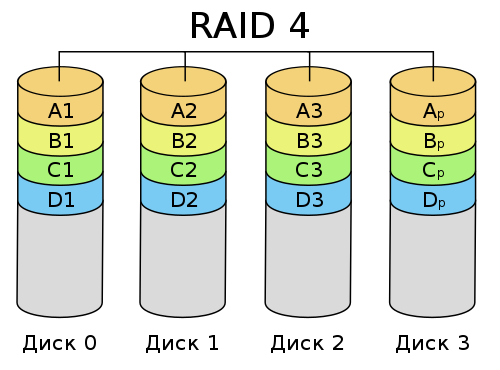
\includegraphics[width=\linewidth]{10/4}}
\end{minipage}
\hfill
\begin{minipage}[h]{0.3\linewidth}
\center{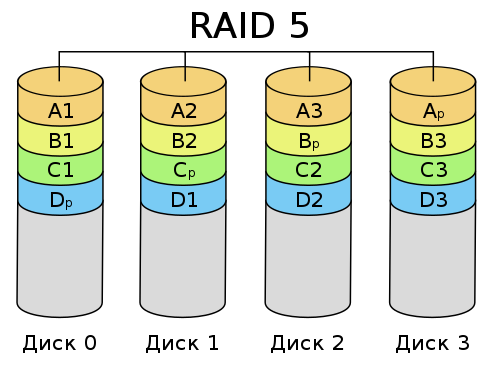
\includegraphics[width=\linewidth]{10/5}}
\end{minipage}
\end{figure}


\item RAID 4. \\
RAID 4 похож на RAID 3, но отличается от него тем, что данные разбиваются на блоки, а не на байты. Таким образом, удалось отчасти "победить" проблему низкой скорости передачи данных небольшого объёма.

\item RAID 5. \\
Та же идея что и в RAID 3, только результат исключающего ИЛИ хранится не на одном конкретном диске (он ведь тоже может сгореть !) а на всех. Например, информация разделена на блоки \\ $A_1, A_2, A_3, B_1, B_2, B_3, C_1, C_2, C_3, D_1, D_2, D_3$, так же:
$A_p = A_1 \oplus A_2 \oplus A_3$, 
$B_p = B_1 \oplus B_2 \oplus B_3$, $C_p = C_1 \oplus C_2 \oplus C_3$, $D_p = D_1 \oplus D_2 \oplus D_3$. Тогда на дисках все будет выглядеть как на картинке: Диск 0 хранит XOR блоков $D_i$, Диск 1 хранит XOR блоков $С_i$, Диск 2 хранит XOR блоков $B_i$, Диск 3 хранит XOR блоков $A_i$. (Остается добавить, что в случае RAID 3 все блоки информации $A_p, B_p, C_p, D_p$ хранились бы на 3 Диске).

Достоинства:
\begin {itemize}
\item RAID 5 получил широкое распространение, в первую очередь благодаря своей экономичности. 
\end {itemize}

Недостатки:
\begin {itemize}
\item Производительность RAID 5 заметно ниже на операциях типа Random Write (записи в произвольном порядке).
\end {itemize}
\end {itemize}
Более подробно можно ознакомится :\href{https://ru.wikipedia.org/wiki/RAID}{RAID}

\subsection {Распределение данных}

\begin{itemize}
\item горизонтальное распределение, когда распределяются данные одного типа. Например, в БД "студенты" данные студентов МГУ хранятся на узле в Москве, а данные студентов СПбГУ - в Санкт-Петербурге; 

\item вертикальное распределение, когда распределяются данные разных типов. Например, в учебной части хранятся оценки, а на кафедре физ.воспитания спортивные достижения;

\item дублирование (т.е. подразумевается непрерывная передача данных между, например, двумя базами). Различают два типа дублирования - синхронное и асинхронное. Про каждый из них ниже.
\end{itemize}

\subsection {Передача данных}
Синхронная передача данных \\
Синхронную передачу применяют в случае, когда базы находятся рядом друг с другом. Принцип работы заключается в том, что фиксация любого изменения происходит с помощью двухфазного коммита. (Заметим, что само состояние двух баз меняется непрерывно, проблема состоит именно в фиксации изменений). \\ 
Модель двухфазного коммита
\begin {itemize}
\item Пользователь заходит на сервер I и делает изменения на сервере I и на сервере II;
\item Пользователь решает зафиксировать свои изменения (операция commit). Сервер I отправляет запрос на сервер II может ли он зафиксировать изменения;
\item Если сервер II отвечает нет (не может зафиксировать), то изменения не фиксируются. Иначе сервер I коммитит изменения у себя и отправляет сообщение серверу II, чтобы он тоже закоммитил изменения у себя; 
\item Сервер II отвечает об успешной фиксации изменений.
\end {itemize}

Асинхронная передача данных \\
В случае, когда серверы находятся далеко друг от друга, пользователь каждый раз при коммите будет долго ждать пока запись "дойдет" до второго сервера. Поэтому используется следующий подход. 
\begin {itemize}
\item Клиент зашел на сервер I и сделал какие-то изменения;
\item Эти изменения не отправляются на сервер II, а пишутся в специальный "журнал"  на сервере I, в котором хранится только то, что изменилось и где;
\item Как только сервер I записал изменения в журнал, пользователь получает сообщение, что изменения закоммичены;
\item Специальный процесс, отправляет на сервер II журнал (например, когда он будет полностью заполнен, хотя может отправлять и чаще);
\item Передача данных завершена.
\end {itemize}